\subsection{Registration}\label{subsec:chp3img-reg:reg}

\begin{figure}
\centering

% Define block styles used later

\tikzstyle{module}=[draw, draw=blue!80, text width=10em, 
    text centered, minimum height=5em, minimum width = 10em, drop shadow, rounded corners,
    fill=blue!30]
    
\tikzstyle{vecArrow} = [thick, decoration={markings,mark=at position
   1 with {\arrow[semithick]{open triangle 60}}},
   double distance=1.4pt, shorten >= 5.5pt,
   preaction = {decorate},
   postaction = {draw,line width=1.4pt, white,shorten >= 4.5pt}]

% Define distances for bordering
\def\blockdist{1.5}
\def\edgedist{2.5}

\definecolor{darkblue}{rgb}{0.2,0.2,0.6}
\definecolor{darkred}{rgb}{0.6,0.1,0.1}
\definecolor{darkgreen}{rgb}{0.2,0.6,0.2}

\def\arrow{
  (10.75:1.1) -- (6.5:1) arc (6.25:120:1) [rounded corners=0.5] --
  (120:0.9) [rounded corners=1] -- (130:1.1) [rounded corners=0.5] --
  (120:1.3) [sharp corners] -- (120:1.2) arc (120:5.25:1.2)
  [rounded corners=1] -- (10.75:1.1) -- (6.5:1) -- cycle
}

\tikzset{
  ashadow/.style={opacity=.25, shadow xshift=0.07, shadow yshift=-0.07},
}

\def\arrows[#1]{         
  \begin{scope}[scale=#1]
	\node[align=center] at (0,0) {\Huge{ Loop } \\ \Huge{ until matching } };  
  
    \draw[color=darkred, %
    drop shadow={ashadow, color=red!60!black}] \arrow;

    \draw[color=darkgreen, bottom color=green!60!black, top color=green!30, %
    drop shadow={ashadow, color=green!60!black}] [rotate=120] \arrow;

    \draw[color=darkblue, right color=blue!60, left color=blue!30, %
    drop shadow={ashadow, color=blue!60!black}] [rotate=240] \arrow;

    % to hide the green shadow
    \draw[color=darkred, left color=red!60, right color=red!30] \arrow;
  \end{scope}
}

%\begin{tikzpicture}[node distance=3cm,thick,path image/.style={
\begin{tikzpicture}[node distance=3cm,thick,scale=0.5, every node/.style={scale=0.5},path image/.style={
path picture={
\node at (path picture bounding box.center) {
\includegraphics[width=1cm]{#1}
};}}]
\tikzstyle{conefill} = [path image=,fill opacity=0.8]

\node (t2w) at (0,0)	{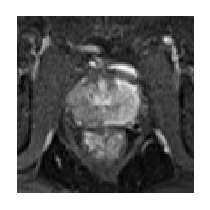
\includegraphics[width=1.5cm]{2_modality/figures/tikzimage/dce.eps}};
\begin{scope}[node distance=1.2cm]
\node[below of=t2w] (cap1) {\Large Fixed};
\end{scope}
\begin{scope}[node distance=6cm]
\node[below of=t2w] 	(dce) 			{\includegraphics[width=1.5cm]{2_modality/figures/tikzimage/t2.eps}};
\begin{scope}[node distance=1.2cm]
\node[below of=dce] (cap2) {\Large Moving};
\end{scope}
\end{scope}

\begin{scope}[node distance=5.5cm]
	\node[module,right of=t2w] (sim) {\Large Similarity \\ measure};
\end{scope}
\begin{scope}[node distance=3cm]
	\node[module,below of=sim] (int) {\Large Interpolator};
	\node[module,below of=int] (tra) {\Large Transform};
\end{scope}

\draw[line width=1mm,draw=blue!30,->] (t2w)--(sim);  
\draw[line width=1mm,draw=blue!30,->] (dce)--(tra); 

\begin{scope}[node distance=9cm]
	\node[module,right of=sim] (opt) {\Large Optimizer};
\end{scope}

\draw[draw=blue,->,line width=.5mm] (tra)--(int);
\draw[draw=blue,->,line width=.5mm] (int)--(sim);
\draw[draw=blue,->,line width=.5mm] (sim)--(opt) node[midway,above] {\Large Similarity} node[midway,below] {\Large metric};
\draw[draw=blue,->,line width=.5mm] (opt)|-(tra); 

\begin{pgfonlayer}{background}
	\path (sim.west |- sim.north)+(-0.5,.5) node (a) {};
    \path (opt.east |- tra.south)+(+0.5,-0.5) node (b) {};
          
    \path[fill=blue!10,rounded corners, draw=blue!20, dashed] (a) rectangle (b);
\end{pgfonlayer} 

\begin{scope}[node distance=5cm]
\node[right of=int] (arr) {
\begin{tikzpicture}
\arrows[1.9];
\end{tikzpicture}
};
\end{scope}
\end{tikzpicture}
\caption[Registration framework.]{Typical framework involved to solve the registration problem.}
\label{fig:frareg}
\end{figure}



%\tikzset{
%  ashadow/.style={opacity=.25, shadow xshift=0.07, shadow yshift=-0.07},
%}
%
%\def\arrows[#1]{         
%  \begin{scope}[scale=#1]
%	\node[align=center] at (0,0) {Loop \\ until \\ matching};  
%  
%    \draw[color=darkred, %
%    drop shadow={ashadow, color=red!60!black}] \arrow;
%
%    \draw[color=darkgreen, bottom color=green!60!black, top color=green!30, %
%    drop shadow={ashadow, color=green!60!black}] [rotate=120] \arrow;
%
%    \draw[color=darkblue, right color=blue!60, left color=blue!30, %
%    drop shadow={ashadow, color=blue!60!black}] [rotate=240] \arrow;
%
%    % to hide the green shadow
%    \draw[color=darkred, left color=red!60, right color=red!30] \arrow;
%  \end{scope}
%}
%
%\begin{tikzpicture}[node distance=3cm,thick,path image/.style={
%path picture={
%\node at (path picture bounding box.center) {
%\includegraphics[width=.5cm]{#1}
%};}}]
%\tikzstyle{conefill} = [path image=,fill opacity=0.8]
%
%\node[inner sep=0pt] (t2w) at (0,0)	{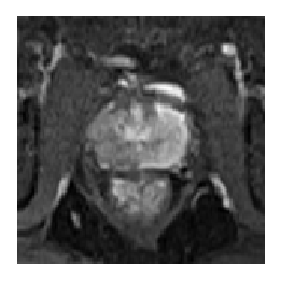
\includegraphics[width=1cm]{02_background/figures/tikzimage/dce.eps}};
%\begin{scope}[node distance=.8cm]
%\node[below of=t2w] (cap1) {Fixed};
%\end{scope}
%\begin{scope}[node distance=3.5cm]
%\node[below of=t2w] 	(dce) 			{\includegraphics[width=1cm]{02_background/figures/tikzimage/t2.eps}};
%\begin{scope}[node distance=.8cm]
%\node[below of=dce] (cap2) {Moving};
%\end{scope}
%\end{scope}
%
%\begin{scope}[node distance=2.5cm]
%	\node[module,right of=t2w] (sim) {Similarity \\ measure};
%\end{scope}
%\begin{scope}[node distance=1.75cm]
%	\node[module,below of=sim] (int) {Interpolator};
%	\node[module,below of=int] (tra) {Transform};
%\end{scope}
%\begin{scope}[node distance=5cm]
%	\node[module,right of=sim] (opt) {Optimizer};
%\end{scope}
%
%\draw[draw=blue,->,line width=.5mm] (tra)--(int);
%\draw[draw=blue,->,line width=.5mm] (int)--(sim);
%\draw[draw=blue,->,line width=.5mm] (sim)--(opt) node[midway,above] {Similarity} node[midway,below] {metric};
%\draw[draw=blue,->,line width=.5mm] (opt)|-(tra);
%
%\draw[line width=.8mm,draw=blue!30,->] (t2w)--(sim);  
%\draw[line width=.8mm,draw=blue!30,->] (dce)--(tra);  
%
%\begin{pgfonlayer}{background}
%	\path (sim.west |- sim.north)+(-0.3,.3) node (a) {};
%    \path (opt.east |- tra.south)+(+0.3,-0.3) node (b) {};
%          
%    \path[fill=blue!10,rounded corners, draw=blue!20, dashed] (a) rectangle (b);
%\end{pgfonlayer} 
%
%\begin{scope}[node distance=3cm]
%\node[right of=int] (arr) {
%\begin{tikzpicture}
%\arrows[1];
%\end{tikzpicture}
%};
%\end{scope}


The role of image registration is vital in \ac{cad} systems using multi-parametric \ac{mri} images. 
As it will be discussed in Sect.~\ref{sec:chp3:img-clas}, for the sake of an optimal classification, the features detected in each modality will be grouped depending of their spatial locations. 
Hence, one has to ensure the perfect alignment of the multi-modal \ac{mri} images ahead of performing any classification.

Image registration is the procedure consisting of aligning an unregistered image (also called moving image) into a template image (also called fixed image) via a geometric transformation.
This problem is usually addressed as presented in Fig.~\ref{fig:frareg}.
An iterative procedure takes place to infer the geometric transformation (parametric or non-parametric) via an optimizer, which maximizes the similarity between the two images.
In the following, a review of the different components of a typical registration framework: transformation model, similarity metric, optimizer and interpolation are presented, followed by a summary of registratio approaches applied in \ac{cad} for \ac{cap} syetems.
Exhaustive reviews covering all registration methods in computer science and medical fields can be found in \cite{Maintz1998} and \cite{Zitova2003}.

%From Sect. \ref{subsubsec:geotra} to \ref{subsubsec:int}, we individually review the different components of a typical registration framework (Fig \ref{fig:frareg}).
%Section \ref{subsubsec:regrev} will summarize the combinations of these components especially for the frameworks used in \ac{cad} systems. 

%% \setenumerate{listparindent=\parindent,itemsep=10px}
%% \setlist{noitemsep}
%% \begin{enumerate}[leftmargin=*]

%\item[$-$] \textbf{\textit{Geometric transformation models:}} 
\paragraph{Geometric transformation models:}
%% From all \ac{cad} for \ac{cap} systems reviewed, only parametric transformation models have been used, mainly based on affine and elastic transformation.
%% Affine transformations provide dgrees of freedom managaing rotations and translation as with the rigid transformations but also shearing and scaling.
As previously mentioned, the registration problem is to align two images or volumes by finding the geometric transformation.
Regarding the transformation, from all \ac{cad} systems reviewed, only parametric methods have been implemented.
Three different groups of parametric transformation models have been used, rigid, affine, and elastic, each of them are characterized by the degree of freedom that they offer.

The first type of transformation is usually referred to as rigid transformation.
These transformations are only composed of rotation and translation transforms.
Hence, for a 2D space where $\mathbf{x} = (x,y) \in \mathbb{R}^2$, a rigid transformation $\mathcal{T}_R$ is formalized as as:

\begin{eqnarray}
	\mathcal{T}_R(\mathbf{x}) & = & \begin{bmatrix}
		R & \mathbf{t} \\
		\mathbf{0^T} & 1
	\end{bmatrix} \mathbf{x} \ , \nonumber \\
	& = & \begin{bmatrix}
		\cos \theta & -\sin \theta & t_x \\
		\sin \theta & \cos \theta & t_y \\
		0 & 0 & 1
	\end{bmatrix}\begin{bmatrix}
		x \\
		y \\
		1
	\end{bmatrix} \ , \label{eq:rigtra} %\\
\end{eqnarray}

\noindent where $\theta$ is the rotation angle and $\{ t_x,t_y \}$ represents the translation along $\{x,y\}$ respectively.

In the case of 3D registration using volume, an additional component $z$ has to be taken into account such that $\mathbf{x} = (x,y,z)$.
Thus, the rotation matrix $\mathbf{R}$ becomes of size $3 \times 3$ whereas the translation vector $\mathbf{t}$ consists of a vector of three elements. 
Hence, the geometric transformation $\mathcal{T}_R(\cdot)$ is embedded into a matrix of size $4 \times 4$.

Affine transformations provide additional degrees of freedom managing rotations and translation as with the rigid transformations but also shearing and scaling.
Hence, for a 2D space where $\mathbf{x} = (x,y) \in \mathbb{R}^2$, an affine transformation $\mathcal{T}_A$ is formalized as: 

\begin{eqnarray}
	\mathcal{T}_A(\mathbf{x}) & = & \begin{bmatrix}
		A & \mathbf{t} \\
		\mathbf{0^T} & 1
	\end{bmatrix} \mathbf{x} \ , \nonumber \\
	& = & \begin{bmatrix}
		a_{11} & a_{12} & t_x \\
		a_{21} & a_{22} & t_y \\
		0 & 0 & 1
	\end{bmatrix}\begin{bmatrix}
		x \\
		y \\
		1
	\end{bmatrix} \ . \label{eq:afftra}% 
\end{eqnarray}
\noindent Hence the four parameters $\{a_{11},a_{12},a_{21},a_{22}\}$ of the affine matrix and $\{ t_x, t_y \}$ of the translation encode an affine transformation.

Regarding volume registeration, the previously mentioned remark can be applied as well.
Thus the geometric transformation $\mathcal{T}_A(\cdot)$ is of size $4 \times 4$ with nine parameters involved.

Finally, the last group of transformations is known as elastic transformations and offer the advantage to handle local distortions.
In the reviewed \ac{cad} systems, the radial basis functions are used to formalize the local distortions such as:

\begin{equation}
	\mathcal{T}_E(\mathbf{x}) = \begin{matrix}
	a_{11} x - a_{12} y + t_x + \sum_i c_i g(\| \mathbf{x} - p_i \|) \\
	a_{21} x + a_{22} y + t_y + \sum_i c_i g(\| \mathbf{x} - p_i \|)
	\end{matrix} \ ,
\end{equation}

\noindent where $\mathbf{x}$ are the control points in both images and $g(\cdots)$ is the actual radial basis function. 

Two radial basis functions are used: (i) the \ac{tps} and (ii) the B-splines.
Apart from the formalism, these two approaches have a main difference: with B-splines, the control points are usually uniformly and densely placed on a grid where as with \ac{tps}, the control points correspond to detected or selected key points.
By using \ac{tps}, Mitra \textit{et al.}~\cite{Mitra2011} obtained more accurate and time efficient results than with the B-splines strategy \cite{Mitra2012a}.

It is reasonable to point out that usually only rigid or affine registrations are used to register multi-parametric images from a same protocol.
Elastic registration methods are more commonly used to register multi-protocol images (e.g., histopathology with \ac{mri} images) \cite{Toth2008,Toth2009}.

%\item[$-$] \textbf{\textit{Similarity measure:}} 
\paragraph{Similarity measure:}
%% During the registration procedure, a similarity criterion is computed in order to evaluate the quality of the alignment performed.
%% Roughly speaking, this criterion will give the direction to take to the optimizer, in order to assign the most optimal values to the geometric transformation parameters.
The most naive similarity measure used in reviewed registration framework is the \acf{mse} of the \ac{si} of \ac{mri} images.
For a pair of images $I$ and $J$, the \ac{mse} is formalized as:

\begin{equation}
	\text{MSE} =\frac{1}{N} \sum_x \sum_y ( I(x,y) - J(x,y) )^2 \ ,
	\label{eq:mse}
\end{equation}
\noindent where $N$ is the total number of pixels.
This metric is not well suited when multi-parametric images are involved due to the tissue appearance variations between the different modalities.

\begin{figure}
\centering
	\hspace*{\fill}
	\subfigure[Illustration of a joint histogram between to aligned image.]{\label{subfig:histoalgn}
\includegraphics[width=0.2\textwidth]{3_review/figures/processing/registration/histogram/jointhistoalg.eps}} \hfill
	\subfigure[Illustration of a joint histogram between to misaligned image.]{\label{subfig:histomisalgn} 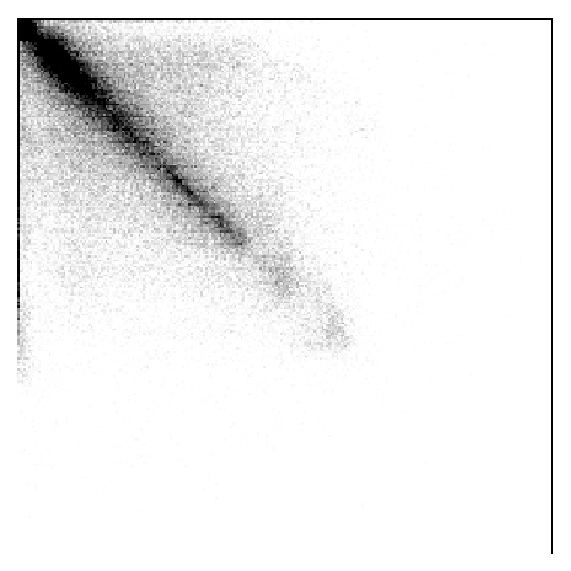
\includegraphics[width=0.2\textwidth]{3_review/figures/processing/registration/histogram/jointhistomisal.eps}}
	\hspace*{\fill}
	\caption[Difference observed in joint histogram between aligned and misaligned images.]{Difference observed in joint histogram between aligned and misaligned images. The joint measure will be more concentrated of the histogram in the case that the images are aligned and more randomly distributed in the case that both images are more misaligned.}
\end{figure}

In that regard, \ac{mi} was introduced as a registration measure in the late 1990's by \cite{Pluim2003}.
The \ac{mi} measure finds its foundation in the assumption that a homogeneous region in the first modality image should also appear as a homogeneous region in the second modality even if their \acp{si} are not identical.
Thus, those regions share information and the registration task can be achieved by maximizing this common information.
Hence, \Ac{mi} of two images $A$ and $B$ is defined as:

\begin{equation}
	MI(A;B) = S(A) + S(B) - S(A,B) \ ,
	\label{eq:midef}
\end{equation}

\noindent where $S(A)$ and $S(B)$ are the marginal entropies and $S(A,B)$ is the joint entropy.
Then, maximizing the \ac{mi} is equivalent to minimizing the joint entropy. 
The joint entropy measure is related with the degree of uncertainty or dispersion of the data in the joint histogram of the images $A$ and $B$.
As shown in Fig.~\ref{fig:jointhisto}, the data in the joint histogram will be concentrated in the case of aligned images while will be more randomly distributed in the case of misaligned images.
Regarding the computation of the entropies, an estimation of the \acp{pdf} have to be carried out.
Histogram or Parzen window methods are a common way to estimate these \acp{pdf}.

A generalized form of \ac{mi}, \ac{cmi}, was proposed by \cite{Chappelow2011}.
\ac{cmi} encompasses interdependent information such as texture and gradient into the metric.
Hence, for both of images $A$ and $B$, the image ensembles $\epsilon^{A}_n$ and $\epsilon^{B}_m$ are generated and composed of $n$ and $m$ images based on the texture and gradient.
Then, the \ac{cmi} can be formulated such as:

\begin{equation}
	CMI(\epsilon^{A}_n;\epsilon^{B}_m) = S(\epsilon^{A}_n) + S(\epsilon^{B}_m) - S(\epsilon^{A}_n,\epsilon^{B}_m) \ .
	\label{eq:cmidef}
\end{equation}

{\color{red} \textbf{Check the commented text, It is not well written and I did not include them}}
%% \noindent From Eq. \eqref{eq:cmidef}, it can be seen that \ac{cmi} is estimated using high dimensional data and that the histogram-based methods to estimate the \acp{pdf} are not suitable any more \cite{Chappelow2011}. 
%% However, other approaches can be used such as the one employed by \cite{Staring2009} to compute the $\alpha$-\ac{mi} \cite{Hero2002}) which is based on the construction of entropic graphs using \ac{knn} inside the high dimensional feature space later used to estimate the \ac{mi}.

%\item[$-$] \textbf{\textit{Optimization methods:}} 
\paragraph{Optimization methods:}
Registration is usually regarded as an optimization problem where the parameters of the geometric transformation model have to be inferred by minimizing the similarity measure.
Iterative estimation methods are commonly used being the L-BFGS-B quasi-Newton method \cite{Byrd1995} and gradient descent \cite{Viola1997} the most common ones. % Nelder-Mead simplex method \cite{Nelder1965},
During our review, we noticed that authors do not usually linger over optimizer choice.

%\item[$-$] \textbf{\textit{Interpolation:}}
\paragraph{Interpolation:} 
The registration procedure involves transforming an image, and pixels mapped to non-integer points must be approximated using interpolation methods.
As for the optimization methods, we notice that little attention has been paid on the choice of those interpolations methods.
However, commonly used methods are bilinear, nearest-neighbour, bi-cubic, spline and inverse-distance weighting method \cite{Mitra2012}.

%\item[$-$] \textbf{\textit{Registration methods used in \ac{cad} systems:}} 
\paragraph{Registration methods used in \ac{cad} systems:}
Studies presenting \ac{cad} pipeline incorporating an automatic registration procedure are summarized in Tab.~\ref{tab:regtab}.

\begin{table}[ht]
  \centering
  \caption{Classification of the different registration methods used in the \ac{cad} systems reviewed. Acronyms: gradient descent (GD), Nelder-Mead (NM).}
  \footnotesize
  %\begin{adjustwidth}{-.1cm}{}
    \begin{threeparttable}
      \renewcommand{\arraystretch}{1}
      \rowcolors{3}{black!5}{white}
      \begin{tabular}{|c|c|c| >{\centering\arraybackslash}m{1.1cm} >{\centering\arraybackslash}m{1.1cm}| >{\centering\arraybackslash}m{0.5cm} >{\centering\arraybackslash}m{0.5cm} >{\centering\arraybackslash}m{0.5cm}| >{\centering\arraybackslash}m{1.1cm} >{\centering\arraybackslash}m{1.35cm}| }\hline
        \hiderowcolors
        Study & Modality & \multirow{2}{*}{Type} & \multicolumn{2}{c|}{Geometric model} & \multicolumn{3}{c|}{Similarity measure} & \multicolumn{2}{c|}{Optimizer} \\ \cline{4-10}
        index & registered & & Affine & Elastic & \acs{mse} & \acs{mi} & \acs{cmi} & GD & L-BFGS-B \\ \hline \hline
        \showrowcolors
        \cite{Ampeliotis2007,Ampeliotis2008} & \ac{t2w} - \ac{dce} & 2D & \cmark & $-$ & \cmark & $-$ & $-$ & $-$ & $-$ \\
        \cite{Giannini2013} & \ac{t2w} - \ac{dw} & 2D & \cmark & \cmark & $-$ & $-$ & $-$ & $-$ & $-$  \\
        \cite{Giannini2013} & \ac{t2w} - \ac{dce} & 2D & \cmark & \cmark & $-$ & \cmark & $-$ & \cmark & $-$ \\
        \cite{Viswanath2008a,Viswanath2009} & \ac{t2w} - \ac{dce} & 2D & \cmark & $-$ & $-$ & \cmark & $-$ & $-$ & $-$ \\
        \cite{Viswanath2011} & \ac{t2w} - \ac{dce} - \ac{dw} & 3D & \cmark & $-$ & $-$ & $-$ & \cmark & \cmark & $-$  \\
        \cite{Vos2008} & \ac{t2w} - \ac{dce} & 3D & \cmark & $-$ & $-$ & \cmark & $-$ & $-$ & $-$ \\
        \cite{Vos2010} & \ac{t2w} - \ac{dce} & 3D & \cmark & \cmark & $-$ & \cmark & $-$ & $-$ & \cmark \\
        \hline
      \end{tabular}
      \begin{tablenotes}
        \footnotesize
      \item Notes:
      \item {$-$}: not used or not mentioned.
      \item {\cmark}: used or implemented.
      \end{tablenotes}
    \end{threeparttable}
\label{tab:regtab}  
%\end{adjustwidth}
\end{table}



Ampeliotis \textit{et al.} in \cite{Ampeliotis2007,Ampeliotis2008} did not use the framework as presented in Fig.~\ref{fig:frareg} to register 2D \ac{t2w} and \ac{dce} images.
By using image symmetries and the \ac{mse} metric, they find the parameters of an affine transformation but without using a common objective function.
They were finding independently and sequentially the scale factor, the rotation and finally the translation.

Giannini \textit{et al.}~\cite{Giannini2013} used also a in-house registration method for 2D \ac{t2w} and \ac{dw} images using an affine model.
The bladder is first segmented in both modalities in order to obtain its contours and to focus the registration.

Giannini \textit{et al.}~\cite{Giannini2013} and also Vos \textit{et al.}~\cite{Vos2010} used the same framework which is based on finding an affine transformation to register the \ac{t2w} and \ac{dce} images using \ac{mi} \cite{Rueckert1999}.
Then, an elastic registration using B-spline takes place using the affine parameters to initialize the geometric model with the same similarity measure.
However, the approaches differ regarding the choice of the optimizer since a gradient descent is used in \cite{Giannini2013} and the same optimization problem is tackled via quasi-Newton method in \cite{Vos2010}.
Moreover, Giannini \textit{et al.}~\cite{Giannini2013} performed a 2D registration whereas Vos \textit{et al.}~\cite{Vos2010} registered 3D volumes.

Viswanath \textit{et al.} in \cite{Viswanath2008a,Viswanath2009} as well as Vos \textit{et al.} \cite{Vos2008} performed an affine registration using the \ac{mi} as similarity measure to correct the misalignment between \ac{t2w} and \ac{dce} images.
The choice of the optimizer was not specified. 
Viswanath \textit{et al.}~\cite{Viswanath2008a,Viswanath2009} focused on 2D registration while Vos \textit{et al.}~\cite{Vos2008} performed 3D registration.

Finally, Viswanath \textit{et al.} in \cite{Viswanath2011} performed a 3D registration with the three modalities, \ac{t2w} and \ac{dce} and \ac{dw} \ac{mri}, by using an affine transformation model combined with the \ac{cmi} similarity measure as presented in \cite{Chappelow2011}.
Moreover, in this latter work, the authors employed gradient descent \cite{Chappelow2011} employed gradient descent approach to solve this problem but suggested Nelder-Mead simplex and quasi-Newton method as other solutions.

%\end{enumerate}
